\chapter{Introducere}

\section{Definiţia anomaliilor}

O \textbf{anomalie} este o entitate ce diferă semnificativ de restul enităţilor din 
setul de date. Definiţia lui Hawkins este urmatoarea\cite{hawkins1980identification}:
\textit{"O anomalie este o observaţie ce deviază atât de mult faţă de restul observaţiilor,
încât să creeze suspiciunea că a fost generată de un mecanism diferit"}.

Datele sunt colectate prin observarea unor procese, de preferat din viaţa reală, 
precum funcţionarea
unui motor sau traficul pe o reţea de calculatoare. În majoritatea timpului, procesele
generează date ce corespund unei derulări normale, dar în anumite cazuri acestea se 
comportă anormal şi astfel apar anomaliile. 

\textit{"Normalitatea"} observaţiilor este definită
de oameni. Algoritmii de învăţare automată pot să semnaleze potenţialele
abateri, dar în final, decizia rămâne a omului.

\section{Caracterizarea anomaliilor nu este viabilă}

Un exemplu ce ilustrează de ce obţinerea de informaţii
despre anomalii este costisitoare ar putea fi activitatea unui
motor defect.

În acest caz, avem 2 variante:
\begin{itemize}
    \item Una dintre ele 
        este să \textbf{simulăm} 
        într-un fel sau altul comportamentul unui motor defectuos, dar 
        se observă că această operaţiune este greu de realizat şi chiar dacă am reuşi 
        să o ducem la capăt, datele colectate nu ar fi autentice şi ar putea duce 
        la o reprezentare incorectă a anomaliilor. 

    \item A doua variantă implică \textbf{sabotarea 
        intenţionată} a motorului pentru a obţine datele, dar acest lucru produce un 
        cost prea mare de cele mai multe ori. 
\end{itemize}

Este evident că definirea anomaliei în acest context nu este viabilă, iar 
cazul nu este singular. Tranzacţiile frauduloase ce constituie tema acestei lucrări 
suferă de aceleaşi probleme, ba mai mult, nici măcar nu avem opţiunea de a 
sabota intenţionat derularea normală a tranzacţiilor. În schimb, 
este mult mai uşor şi cel mai probabil 
implică un cost aproape inexistent, să urmărim activitatea unui motor 
în stare bună de funcţionare şi să folosim datele respective pentru a 
defini ce înseamnă o observaţie normală.

\section{Aplicaţii ale detecţiei anomaliilor}

\begin{itemize}
    \item \textbf{Fraude financiare}: ne dorim să semnalăm comportamentul ciudat 
    observat într-o serie de tranzacţii, precum activitatea generată de 
    o persoana care foloseşte cardul de credit al altei persoane în mod 
    neautorizat. Această aplicaţie constituie şi obiectul lucrării noastre.
    \item \textbf{Intruziune în reţele de calculatoare}: vrem să semnalăm activitatea
    neobişnuită ce poate indica un potenţial atac cibernetic sau accesul 
    neautorizat al unui terţ maliţios.
    \item \textbf{Controlul calităţii în manufactură}: suntem interesaţi să monitorizăm 
    procesul de producţie pentru a raporta eventualele defecţiuni ce ar afecta 
    calitatea produsului.
    \item \textbf{Domeniul medical}: vrem să identificăm anomalii în analizele de sânge, 
    semnele vitale sau imaginile medicale ale pacientului pentru a depista şi preveni
    anumite afecţiuni.
    \item \textbf{Reţele sociale}: ne dorim să raportăm automat conţinutul postat ce 
    poate include remarci jignitoare, precum comentariile rasiste sau xenofobe,
    astfel fiind de ajutor în moderarea materialului încărcat pe platforme. 
\end{itemize}

\section{Tipuri de detecţie a anomaliilor}

\subsection{Outlier detection}

\textbf{Outlier detection} are scopul de a identifica observaţii fie noi,
fie previzibile, din setul de antrenare, care deviază de la 
comportamentul normal. 
\textbf{Outliers} pot fi valori extreme, erori cauzate 
de zgomot, posibil din instrumentele de măsură sau senzorii folosiţi 
pentru colectarea datelor, sau comportament anormal.

Această abordare este utilă atunci când avem un set de date \textbf{"poluat"} cu 
observaţii anormale şi ne dorim să extragem din el doar porţiunea ce conţine 
observaţii deviante. De asemenea, se poate folosi atât pe seturi adnotate, cât 
şi pe seturi fără etichete.

\subsection{Novelty detection}

\textbf{Novelty detection} are scopul de a identifica observaţii noi 
ce diferă semnificativ de datele de antrenare care au rolul de a 
caracteriza cât mai bine clasa normală. Din acest motiv, este foarte 
important ca setul de antrenare să nu conţină
decât date normale pentru a putea identifica caracteristicile clasei de referință,
astfel modelând comportamentul normal.

Prin urmare, această abordare este utilă atunci cand avem un 
set de date \textbf{"curat"} (fără 
anomalii) şi ne aşteptăm ca observaţiile noi să fie rare şi să aibă trăsături
distincte faţă de setul de antrenare. De asemenea, se presupune că datele sunt adnotate 
pentru a putea extrage punctele cu eticheta normală şi să le folosim la antrenare.

\textbf{Novelty detection} este tipul de detecţie al anomaliilor pe care îl studiem în 
această lucrare.

\section{Detecţia anomaliilor vs clasificare binară}

\subsection{Greşeală comună}

La prima vedere, aceste două probleme par sa coincidă şi ne determină
să ne întrebăm de ce a mai apărut un nou domeniu de cercetare, anume detecţia
anomaliilor, când deja avem la dispoziţie atâtea rezultate utile pentru 
problema clasificării. Un argument ar putea fi că 
detecţia anomaliilor este de fapt o problemă de clasificare binară în care proporţia
celor 2 clase este neechilibrată. Deşi este contraintuitiv, această 
afirmaţie este greşită.

\subsection{Scopul detecţiei anomaliilor}

Diferenţa constă în faptul că detecţia anomaliilor are la bază \textbf{o singură clasă
de referință}. Observaţia fie aparţine acestei clase, fie aparţine oricărei alte clase 
care este diferită de aceasta din urmă. Multitudinea de "clase diferite" ne indică
faptul că este greu să definim ce înseamnă \textit{"diferit de normal"}, dar este relativ uşor
să definim ce înseamnă \textit{"normal"}.

Un exemplu trivial ar putea fi să detectăm dacă animalul din imagine este un câine sau nu.
În acest caz, normal înseamnă câine, iar anormal înseamnă orice alt animal care nu este
câine. Se observă că este relativ uşor să caracterizăm conceptul de câine, în timp ce 
definirea conceptului de "diferit de câine" este complexă, fapt ce ar pune în dificultate
un clasificator binar care prin definiţie învaţă trăsăturile definitorii pentru ambele 
clase. 

\subsection{Scopul clasificării binare}

La clasificarea binară, cele 2 clase sunt bine 
definite şi de cele mai multe ori, trasăturile lor se suprapun în mai multe locuri. De 
asemenea, această problemă acordă o importanţă \textbf{egală} celor 2 categorii, pe când
eşecul de a semnala o anomalie este în general mult mai dăunător faţă de 
detectarea unei observaţii normale ca fiind anormală. 

Pentru a continua exemplul precedent cu imaginile cu animale, putem reformula problema 
ca de această dată să diferenţiem între pisici şi câini. Deja se vede că ambele clase 
sunt mult mai bine definite şi putem găsi atât trăsături comune, precum nasul, cât şi 
trăsături definitorii, precum mustăţile. Vrem să detectăm la fel de bine ambele animale, 
pe când într-o problemă clasică de detecţie a anomaliilor, precum identificarea 
tranzacţiilor frauduloase, vrem preponderent să nu ratăm evenimentele cu 
caracter maliţios.


\begin{figure}[H]
    \centering
    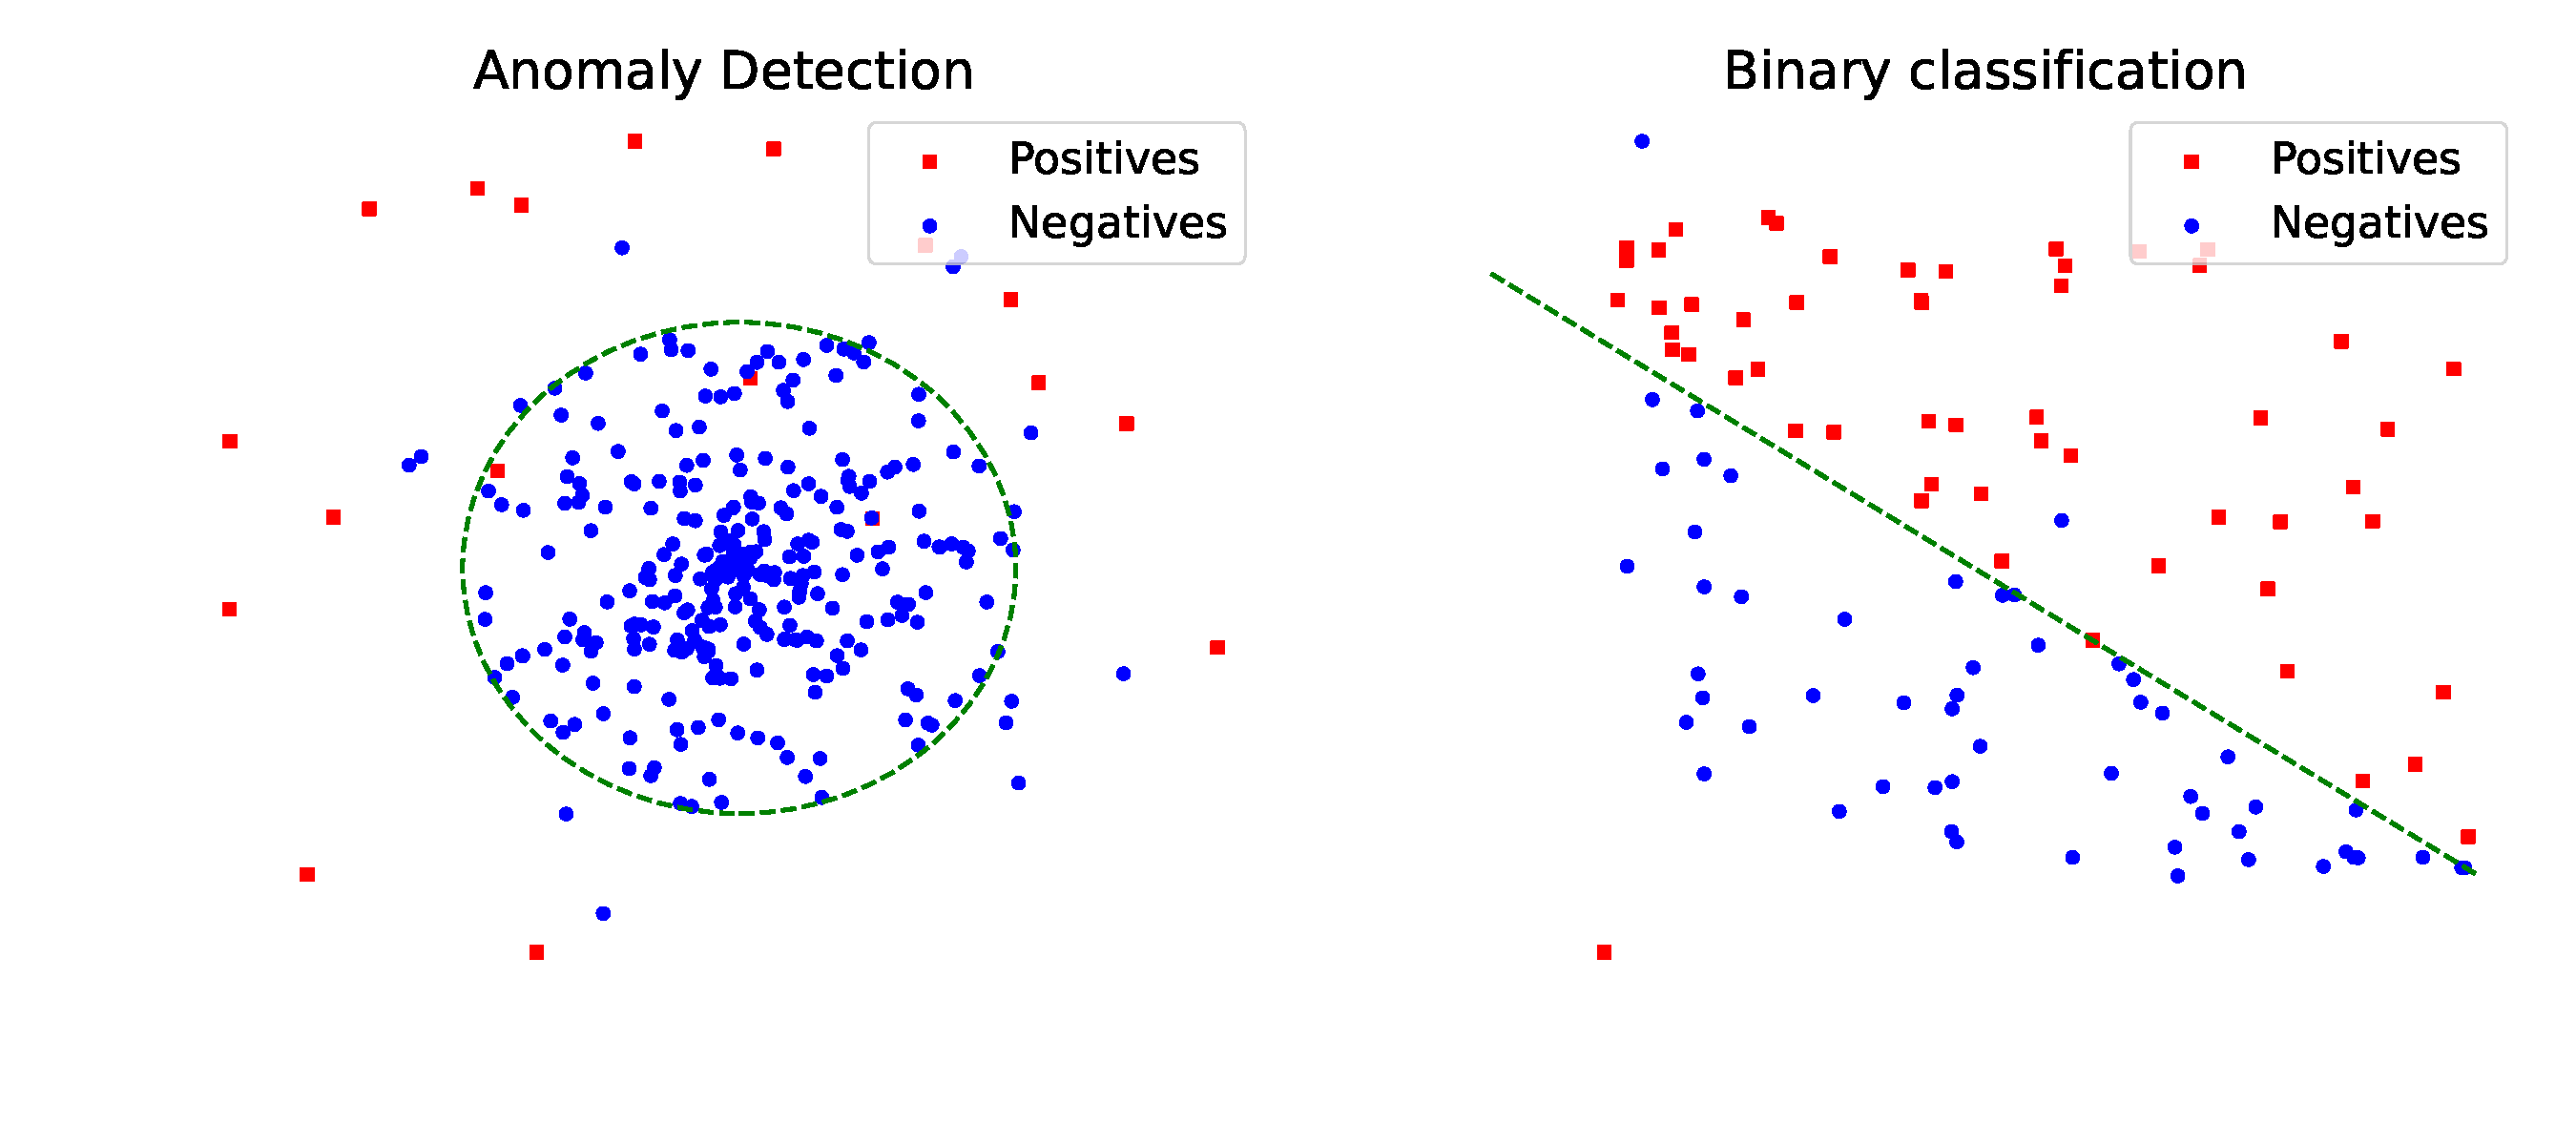
\includegraphics[width=\linewidth]{images/The-anomaly-detection-and-the-classification-learning-schemas.pdf}
    \caption{Detecţia anomaliilor în stânga şi clasificarea binară în dreapta}
\end{figure}